\documentclass[11pt, onecolumn, oneside, reqno]{amsart}
\usepackage[english]{babel}

\usepackage{geometry}
\geometry{a4paper}

\usepackage[parfill]{parskip}
\usepackage[pdftex]{graphicx}	

\usepackage[font=small]{caption}
\usepackage[font=small]{subcaption}

% source code listings in C++
\usepackage{listings}
\lstset{frame=single, language=C++, basicstyle=\footnotesize}

% hyperref should be the last package declaration
\usepackage[colorlinks=true, urlcolor=blue, linkcolor=green]{hyperref}

\title{Udacity Project: Deep RL Arm Manipulation}
\author{Stephan Hohne}
\date{May 29, 2018}

\begin{document}
\maketitle

\section{Introduction}
This is a solution of the \href{https://github.com/udacity/RoboND-DeepRL-Project}{Deep RL Arm Manipulation} project as part of the Robotics Nanodegree. The goal of the project is to set up and optimize a reinforcement learning framework. A Deep Q-Network learns to control a robotic arm in a simulated Gazebo environment. The reinforcement learning agent is given the task of touching a target object.
\begin{description}
\item[Objective 1] Have any part of the robot arm touch the object of interest, with at least a $90\%$ accuracy for a minimum of $100$ runs.
\item[Objective 2] Have only the gripper base of the robot arm touch the object, with at least a $80\%$ accuracy for a minimum of $100$ runs.
\end{description}

The project tasks were to implement parts of the \href{https://github.com/S2H-Mobile/RoboND-DeepRL-Project-Solution/blob/develop/gazebo/ArmPlugin.cpp}{ArmPlugin.cpp} file, see section \ref{sec:simulations}. The reward function was to be designed (section \ref{sec:reward-function-design}), and the DQN hyper-parameters were to be tuned (section \ref{sec:dqn_parameter_tuning}).

The network training along with the simulation runs were performed on the Udacity Project Workspace with enabled GPU.
 
\section{Simulations}
\label{sec:simulations}
Before running simulation experiments, the following parts of the \href{https://github.com/S2H-Mobile/RoboND-DeepRL-Project-Solution/blob/develop/gazebo/ArmPlugin.cpp}{ArmPlugin.cpp} file were implemented.
\begin{itemize}
\item The subscription to camera and collision topics.
\item The creation of the DQN agent using learning hyperparameters defined as constants in the file.
\item The definition of collision checks to determine which robot arm link touched the target object.
\item Both velocity control and position control of the robot were implemented.
\item Criteria for ground contact of the arm were defined, see listing \ref{fig:listing_ground_contact}. The $z$-coordinates of the gripper link bounding box were used. The threshold ground level was set at $z=0.05$ meters to accommodate for the inaccuracy of the distance calculation.
\end{itemize}

\begin{figure}[thpb]
\centering
\begin{lstlisting}
// define the z value for  ground contact
const float groundContact = 0.05f;

// define condition for ground contact
const bool checkGroundContact =
	( gripBBox.min.z <= groundContact
	|| gripBBox.max.z <= groundContact );
\end{lstlisting}
\caption{Criteria for ground contact of the gripper base link.}
\label{fig:listing_ground_contact}
\end{figure}

Several experimental runs of the simulation were performed, testing different versions of the reward function and tuning the DQN parameters.

\subsection{Reward Function Design}
\label{sec:reward-function-design}
A reward system was set up in order to teach the robotic arm how to reach for the target object. Positive and negative rewards are defined as numeric constants \texttt{REWARD\_WIN} and \texttt{REWARD\_LOSS}. A win is issued for touching the prop with any link (objective 1) or the gripper base link (objective 2). A loss is issued when the arm touches the ground or when the length of the episode exceeds $100$ steps in time. The occurrence of any of these events will end the episode.

Since positive rewards from touching the prop by the gripper link are very sparse, an interim reward function was designed. Its purpose is to guide the robot arm towards the target. The relevant measure is the distance $d_t$ between gripper and target object. For consecutive steps $t-1$ and $t$, the difference $\Delta_t = d_{t-1} - d_t$ was calculated. In order to obtain a smooth reward function, the moving average of the recorded $\Delta$ values was computed, see listing \ref{fig:source_smoothed_moving_average}. 
\begin{figure}[htpb]
\centering
\begin{lstlisting}
const float distDelta  = lastGoalDistance - distGoal;

avgGoalDelta  = (avgGoalDelta * ALPHA) + (distDelta * (1.0f - ALPHA));
\end{lstlisting}
\caption{Code for computing the delta of the distance to goal and the corresponding smoothed moving average. The value of the alpha parameter is a constant that was tuned in the experiments.}
\label{fig:source_smoothed_moving_average}
\end{figure}

A linear function of the \texttt{avgGoalDelta} function is proportional to the average speed towards the goal and should be a good candidate for the interim reward function, see for example \ref{fig:linear_reward_function_objective_2}. The parameter values found in the experiments are shown in table \ref{tab:reward_params_objectives}.

\subsubsection{Objective 1}
Velocity control of the robot arm was enabled during the simulation runs. Two versions of a reward function were tested, see  figure \ref{fig:reward_functions_objective_1} for the source code. The first version is a linear function proportional to the moving average. The second version issues different rewards, depending on the sign of \texttt{avgGoalDelta}. The positive reward is the same as in version 1, the negative reward is proportional to the goal distance.  

\begin{table}[thpb]
	\centering
	\renewcommand{\arraystretch}{1.3}
	\begin{tabular}{|l|c|c|c|}
	\hline
	Experiment & 1 & 2 & 3 \\
	\hline
	Reward function, see \ref{fig:reward_functions_objective_1}  & version 1 &  version 2 &  version 2 \\
	\hline
	\multicolumn{4}{|l|}{Best run} \\ 
	\hline
	Accuracy / episodes & $0.9694 / 98$ & $0.9466 / 131$ & $0.9800 / 100$ \\
	\hline
	\end{tabular}
	\caption{Experimental runs for objective 1. See figure \ref{fig:objective_1_achieved} for an image showing the result of experiment 3.}
	\label{tab:experiments_objective_1}
\end{table}

\begin{figure}[htpb]
\centering
\begin{lstlisting}
// version 1
rewardHistory = INTERIM_REWARD * avgGoalDelta;

// version 2
rewardHistory = avgGoalDelta > 0 
	? INTERIM_REWARD * avgGoalDelta
	: REWARD_LOSS * distGoal;
\end{lstlisting}
\caption{Implementation of two versions of the reward function. The value of the reward loss is $-10.0$, and the value of the interim reward is $10.0$, see table \ref{tab:reward_params_objectives}.}
\label{fig:reward_functions_objective_1}
\end{figure}

Both versions of the interim reward function met objective 1, see table \ref{tab:experiments_objective_1} and section \ref{sec:results}. The fixed configuration of the DQN agent used during the experimental runs is shown in figure \ref{fig:fixed_dqn_params_objective_1}.

\subsubsection{Objective 2}
The reward parameters and agent control were adjusted following advice from students on Slack community channel.
\begin{itemize}
\item The velocity control was switched to position control.
\item The value of the moving average \texttt{ALPHA} was lowered from the initial guess of $0.9$ to values in the range $\left[0.4, 0.5\right]$.
\end{itemize}

In order to explore alternatives to the linear reward function, the effect of an exponential function of the distance of the form
\begin{equation}
\label{eqn:exponential_damping}
\gamma \left(\mathtt{distGoal}\right) = \exp \left( -\beta \, \mathtt{distGoal} \right)
\end{equation}
with $\beta \in \mathbb{R}$ was studied. An exponential factor with $\beta = -1.0$ was applied to the reward function, see listing \ref{fig:exponential_damping_reward}. Since the range is $\gamma  \in \left[0, 1\right]$, the reward should be damped with increasing distance, making gripper positions close to the target object more desirable. In the experimental runs the arm accelerated towards the target objective and failed to accomplish the task.

\begin{figure}[thpb]
\centering
\begin{lstlisting}
rewardHistory = exp(-1.0f * distGoal) * INTERIM_REWARD * avgGoalDelta;
\end{lstlisting}
\caption{Implementation of the exponential damping factor \ref{eqn:exponential_damping} as part of the interim reward function.}
\label{fig:exponential_damping_reward}
\end{figure}

The exponential \ref{eqn:exponential_damping} with $\beta = -1.0$ was also used in the calculation of the moving average as a replacement of the constant alpha parameter, see listing \ref{fig:exponential_damping_moving_average}. The intention was to give less weight to distance deltas when the arm is close to the target object. This should accommodate for the inaccuracy in the computation of small distance deltas. In the experimental runs the arm slowed down to a halt before reaching the target objective and failed to accomplish the task. It is left to future work to investigate the use of exponential reward functions further.

\begin{figure}[thpb]
\centering
\begin{lstlisting}
const float gamma = exp(-1.0f * distGoal);
avgGoalDelta  = (avgGoalDelta * gamma) + (distDelta * (1.0f - gamma));
rewardHistory = 40.0f * avgGoalDelta;
\end{lstlisting}
\caption{Implementation of the exponential damping factor \ref{eqn:exponential_damping} in the computation of the moving average.}
\label{fig:exponential_damping_moving_average}
\end{figure}

In subsequent experiments, a linear reward function was used again, see listing \ref{fig:linear_reward_function_objective_2}. A negative offset was introduced to punish standstill or the moving away from the target. The parameters \texttt{INTERIM\_REWARD} and \texttt{INTERIM\_OFFSET} represent the slope and the offset, respectively. These parameters, together with the alpha parameter of the moving average were tuned experimentally, see table \ref{tab:reward_param_tuning_objective_2}. During the experiments, \texttt{REWARD\_WIN} was set to $20.0$, and \texttt{REWARD\_LOSS} was set to $-20.0$.  The configuration of the DQN agent used during the experimental runs is shown in table \ref{tab:reward_param_tuning_objective_2} and figure \ref{fig:fixed_dqn_params_exp_3_objective_2}. Objective 2 was met using the linear reward function.

\begin{figure}[thpb]
\centering
\begin{lstlisting}
// linear reward function
rewardHistory = INTERIM_REWARD * avgGoalDelta - INTERIM_OFFSET;
\end{lstlisting}
\caption{Code for the interim reward function as a linear function of the moving average. The parameters \texttt{INTERIM\_REWARD} and \texttt{INTERIM\_OFFSET} are constants that were tuned in the experiments.}
\label{fig:linear_reward_function_objective_2}
\end{figure}

\begin{table}[thpb]
	\centering
	\renewcommand{\arraystretch}{1.3}
	\begin{tabular}{|l|r|r|r|}
	\hline
	Experiment & 1 & 2 & 3 \\
	\hline
	\texttt{LEARNING\_RATE} & $0.1$  & $0.08$ & $0.1$  \\
	\texttt{BATCH\_SIZE}    & $32$   & $256$  & $256$  \\
	\texttt{EPS\_START}     & $0.9$  & $0.7$  & $0.7$  \\
	\texttt{EPS\_END}       & $0.05$ & $0.02$ & $0.02$ \\
	\hline
	\texttt{INTERIM\_REWARD} & $4.0$ & $4.0$ & $4.0$ \\
	\texttt{INTERIM\_OFFSET} & $0.2$ & $0.2$ & $0.3$ \\
	\hline
	\texttt{ALPHA} & $0.5$ & $0.5$ &  $0.4$\\
	\hline
	\multicolumn{4}{|l|}{Best run} \\ 
	\hline
	Accuracy / episodes & $0.8070 / 715$ &  $0.8125 / 352$ & $0.8202 / 228$ \\
	\hline
	\end{tabular}
	\caption{Parameter tuning for achieving objective 2. The linear reward function \ref{fig:linear_reward_function_objective_2} was used.}
	\label{tab:reward_param_tuning_objective_2}
\end{table}


\subsection{DQN Hyperparameter Tuning}
\label{sec:dqn_parameter_tuning}
The size of the input was set to $64 \times 64$, since the camera image sent to the agent is of that size. The long-short-term memory was enabled by setting \texttt{LSTM} constant to true. The \texttt{RMSprop} and the \texttt{Adam} optimizer \cite{adam_paper} were tested. \texttt{RMSprop} was used during the simulation runs for objective 1, \texttt{Adam} was used in the reward function design experiments for objective 2. When going from objective 1 to objective 2, the batch size was increased from $32$ to $256$, see \ref{fig:dqn_params}. The LSTM size was increased from $64$ to $256$, which should allow the agent to memorize more complex moves. 

During the simulation runs for objective 2 (see table \ref{tab:reward_param_tuning_objective_2}), the start value of the exploration parameter \texttt{EPS\_START} was tuned between the values $0.9$ and $0.7$. The end value of the exploration parameter \texttt{EPS\_END} was tuned between the values $0.05$ and $0.02$. The learning rate was tuned between the values $0.08$ and $0.1$. The performance of each configuration was determined using the accuracy output during the simulations.

\begin{figure}[thpb]
\centering
\begin{subfigure}{.49\textwidth}
\begin{lstlisting}
// Define DQN API Settings
#define INPUT_CHANNELS 3
#define ALLOW_RANDOM true
#define DEBUG_DQN false
#define GAMMA 0.9f
#define EPS_START 0.7f
#define EPS_END 0.02f
#define EPS_DECAY 200

// Define Learning Hyperparameters
#define INPUT_WIDTH   64
#define INPUT_HEIGHT  64
#define OPTIMIZER "RMSprop"
#define LEARNING_RATE 0.1f
#define REPLAY_MEMORY 10000
#define BATCH_SIZE 32
#define USE_LSTM true
#define LSTM_SIZE 64
\end{lstlisting}
\caption{Experiments for objective 1.}
\label{fig:fixed_dqn_params_objective_1}
\end{subfigure}
\begin{subfigure}{.49\textwidth}
\begin{lstlisting}
// Define DQN API Settings
#define INPUT_CHANNELS 3
#define ALLOW_RANDOM true
#define DEBUG_DQN false
#define GAMMA 0.9f
#define EPS_START 0.7f
#define EPS_END 0.02f
#define EPS_DECAY 200

// Define Learning Hyperparameters
#define INPUT_WIDTH   64
#define INPUT_HEIGHT  64
#define OPTIMIZER "Adam"
#define LEARNING_RATE 0.1f
#define REPLAY_MEMORY 10000
#define BATCH_SIZE 256
#define USE_LSTM true
#define LSTM_SIZE 256
\end{lstlisting}
\caption{Experiment 3 for objective 2.}
\label{fig:fixed_dqn_params_exp_3_objective_2}
\end{subfigure}
\caption{DQN configurations used during the reward function experiments.}
\label{fig:dqn_params}
\end{figure}

\section{Results}
\label{sec:results}
Both objectives were achieved. The best performing runs were observed with the linear reward function \ref{fig:linear_reward_function_objective_2}, while the exponential reward function did not meet the objectives.

The largest positive effect on the agents performance was observed when lowering the value of the moving average \texttt{ALPHA} parameter from $0.9$ to $0.4$, see section \ref{sec:reward-function-design}. This finding emphasizes the importance of designing a smooth reward function.

The best performing configurations for each objective are shown in table \ref{tab:reward_params_objectives}. The number of episodes it took the agent to reach the threshold accuracy varied between $\approx 200$ and $\approx 700$, depending on the initial conditions of the simulation run. During the simulation runs, the accuracy improved slowly over time. For example, after taking screenshot \ref{fig:objective_2_achieved} the accuracy of that run went up to over $83\%$ after $\approx 260$ episodes.

\begin{table}[thpb]
	\centering
	\renewcommand{\arraystretch}{1.3}
	\begin{tabular}{|l|r|r|}
	\hline
	Objective & 1 & 2  \\
	\hline
	\texttt{REWARD\_WIN}   & $10.0$ & $20.0$  \\
	\texttt{REWARD\_LOSS}   & $-10.0$ & $-20.0$  \\
	\hline
	\texttt{INTERIM\_REWARD}   & $10.0$ & $4.0$  \\
	\texttt{INTERIM\_OFFSET}   & n.\ a. & $0.3$  \\
	\hline
	\texttt{ALPHA}   & $0.9$ & $0.4$  \\
	\hline
	\multicolumn{3}{|l|}{Best run} \\ 
	\hline
	Accuracy / episodes & $0.9800 / 100$  & $0.8202 / 228$ \\
	\hline
	Image &  \ref{fig:objective_1_achieved} &  \ref{fig:objective_2_achieved} \\
	\hline
	\end{tabular}
	\caption{Values of reward parameters for the best performing simulation runs, achieving objectives 1 and 2.}
	\label{tab:reward_params_objectives}
\end{table}

\begin{figure}[htpb]
      \centering
      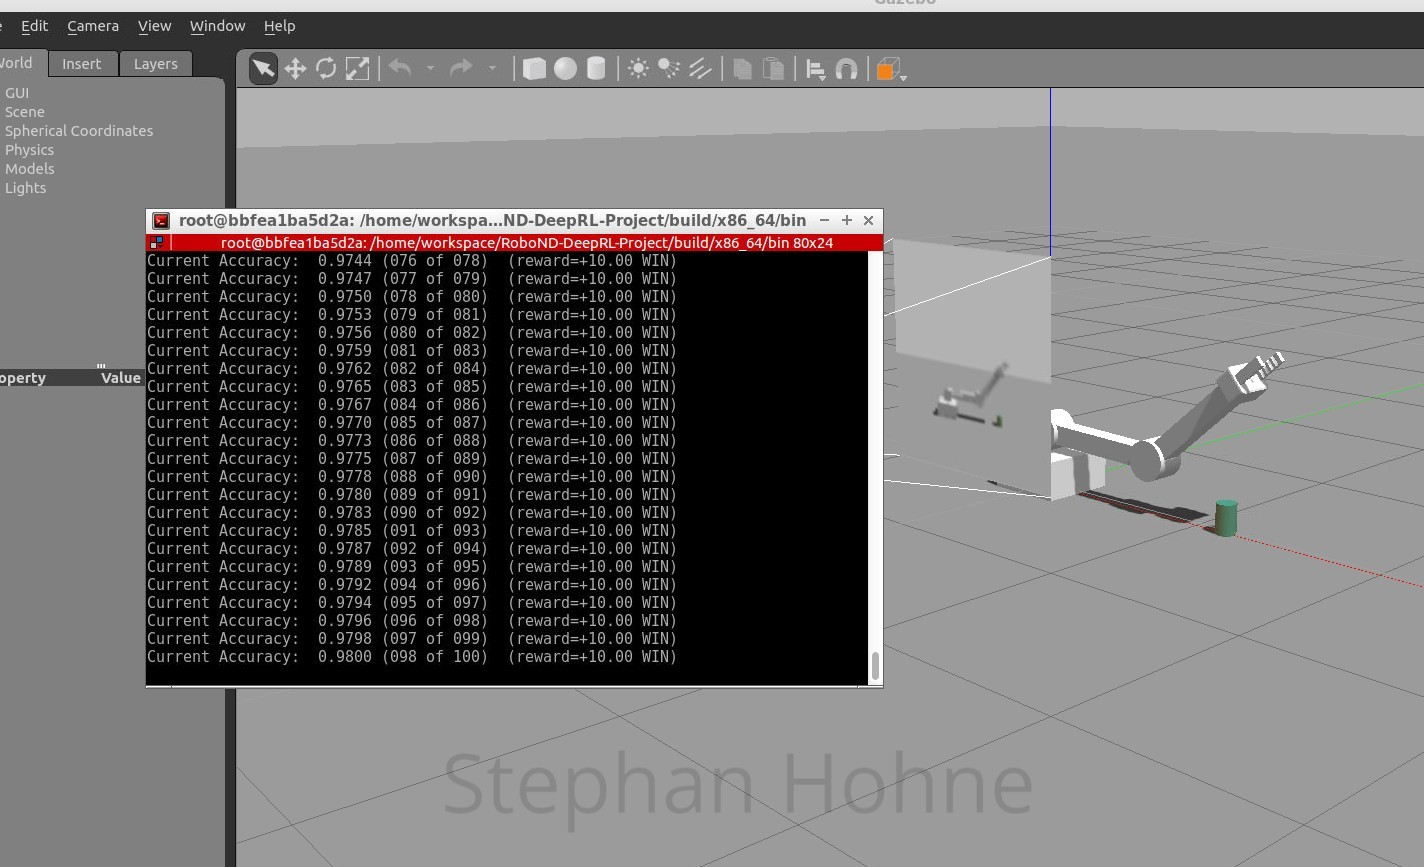
\includegraphics[width=\linewidth]{images/100_signed.PNG}
      \caption{Simulation run that achieved objective 1. See experiment 3 in table \ref{tab:experiments_objective_1}.}
      \label{fig:objective_1_achieved}
\end{figure}

\begin{figure}[htpb]
      \centering
      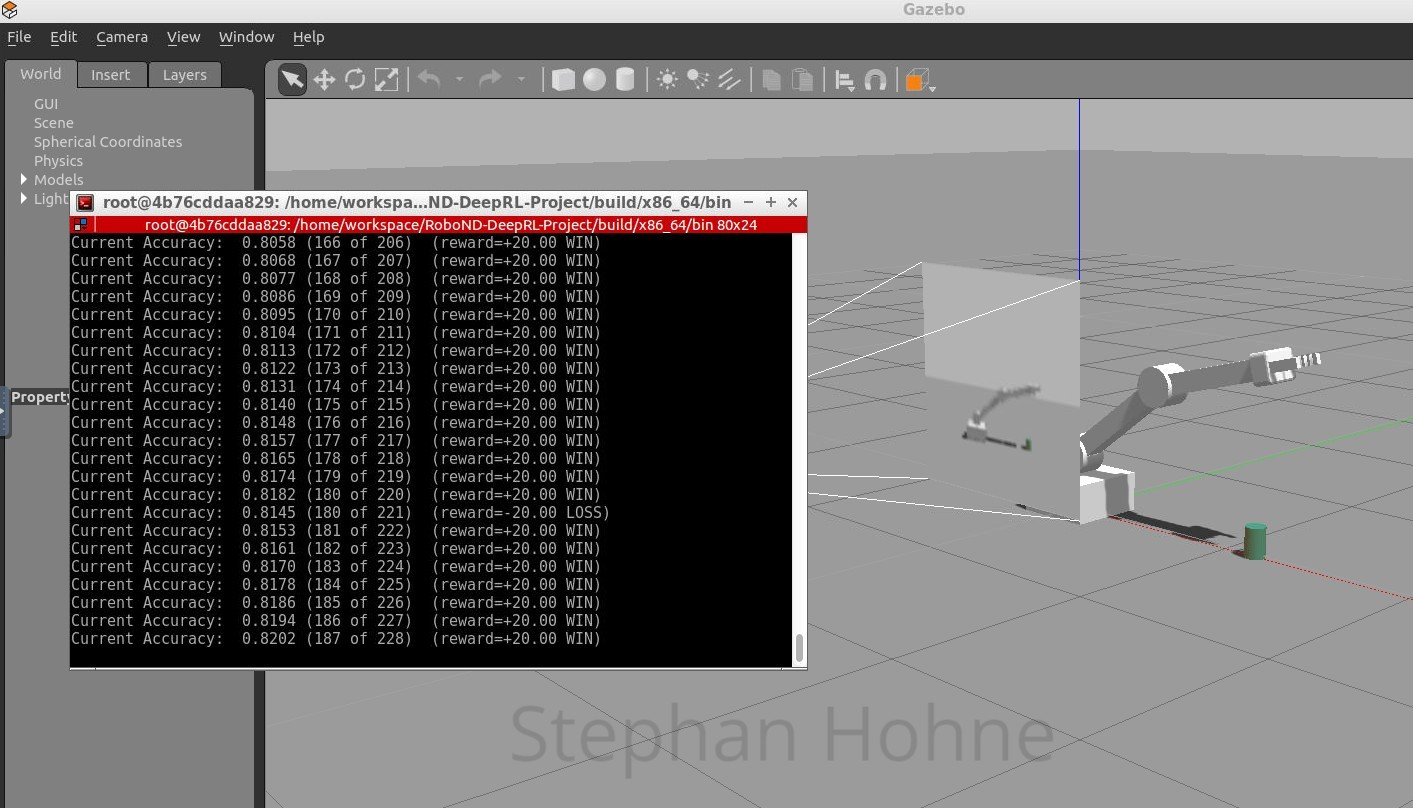
\includegraphics[width=\linewidth]{images/228_signed.PNG}
      \caption{Simulation run that achieved objective 2. See experiment 3 in table \ref{tab:reward_param_tuning_objective_2}.}
      \label{fig:objective_2_achieved}
\end{figure}

\section{Future Work}
The reinforcement-learning framework can be improved further by:
\begin{itemize}
\item Tuning the remaining DQN hyperparameters like the discount factor, size of replay memory, and epsilon decay rate.
\item Investigating whether the exponential damping function \ref{eqn:exponential_damping} can be improved to create a reward function able to achieve the objectives. 
\end{itemize}

Additionally, the plan is to let the project run on the Jetson TX2. It will also be interesting to see how well the framework generalizes to controlling a robotic arm with enhanced capabilities and more degrees of freedom.

\begin{thebibliography}{1}
\bibitem{adam_paper}
Diederik P. Kingma and Jimmy Ba, \textit{Adam: {A} Method for Stochastic Optimization}, CoRR, 2014, \href{http://arxiv.org/abs/1412.6980}{arXiv  abs/1412.6980}
\end{thebibliography}

\end{document}